\documentclass[10pt]{beamer}
\usepackage{verbatim}
\usepackage{amsmath}
\usepackage{amsthm}
\usepackage{graphics}
\usepackage{color}
\usepackage{stmaryrd}\usefonttheme[onlymath]{serif}

\title{Discussion 2}
\date{\today}

\begin{document}
\maketitle


\begin{frame}\frametitle{Crucial Problem}
Different from the disjunctive invariant problem, which only needs to generate a max-plus convex to surround the samples, the dependcy relation between different parts is much more important in multiphase ranking function.

So the crucial problem is to find a effective way to split these areas.

\end{frame}


\begin{frame}\frametitle{Idea1: Blocks}
Use disjunctive terms of the loop guards and branch guard for multiphase ranking function.
\begin{center}
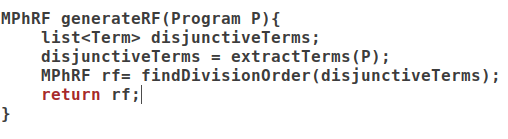
\includegraphics[scale=0.5]{2.png}
\end{center}
This algorithm is unsound because..
\end{frame}


\begin{frame}\frametitle{Unsound example}
\begin{example}

\[\texttt{while }(x > 0 \vee y > 0) \]
\[\{\texttt{if }(y > 0): y' = y - 1; x' = 5;\]
\[\texttt{else }: x' = x - 1; y = 5; \}\]


\end{example}
$\neg(y > 0) \wedge (x > 0 \vee y > 0) = x > 0$
\end{frame}

\begin{frame}\frametitle{Idea2}
Let $\mathcal{Q}$ be the state space of the loop.
Use SVMRanker to learn a nested function except removing constraint $f_d(x) \ge 0$.
After learning, we get a set of function $\{f_1,\ldots, f_d\}_1$ which is decreasing in the whole space.

If the state space lies in $f_d(x) \ge 0$, then we finished. Otherwise,
For transitions $(x, x')$ where $x \in \mathcal{Q}\cap \{x\mid f_d(x) > 0\}_1$, $(x, x')$ is ranked by $f_1(x)$ and we repeat the procedure recursively to find $\{f_i\}_2, \{f_i\}_3\ldots$.
\begin{example}

\[\texttt{while }(x > 0 \vee y > 0) \]
\[\{\texttt{if }(y > 0): y' = y - 1; x ' = x;\texttt{else }: x' = x - 1;\}\]
\end{example}

First find $y$, because for the whole space $y$ is always decreasing or remain unchanged and use $y \ge 0$ to reduce the loop.
Then find $x$, as the second phase ranking function for it is also always decreasing in $Q\cap \{y < 0\}$.
\end{frame}


%\begin{frame}\frametitle{Idea3}

%\begin{center}
%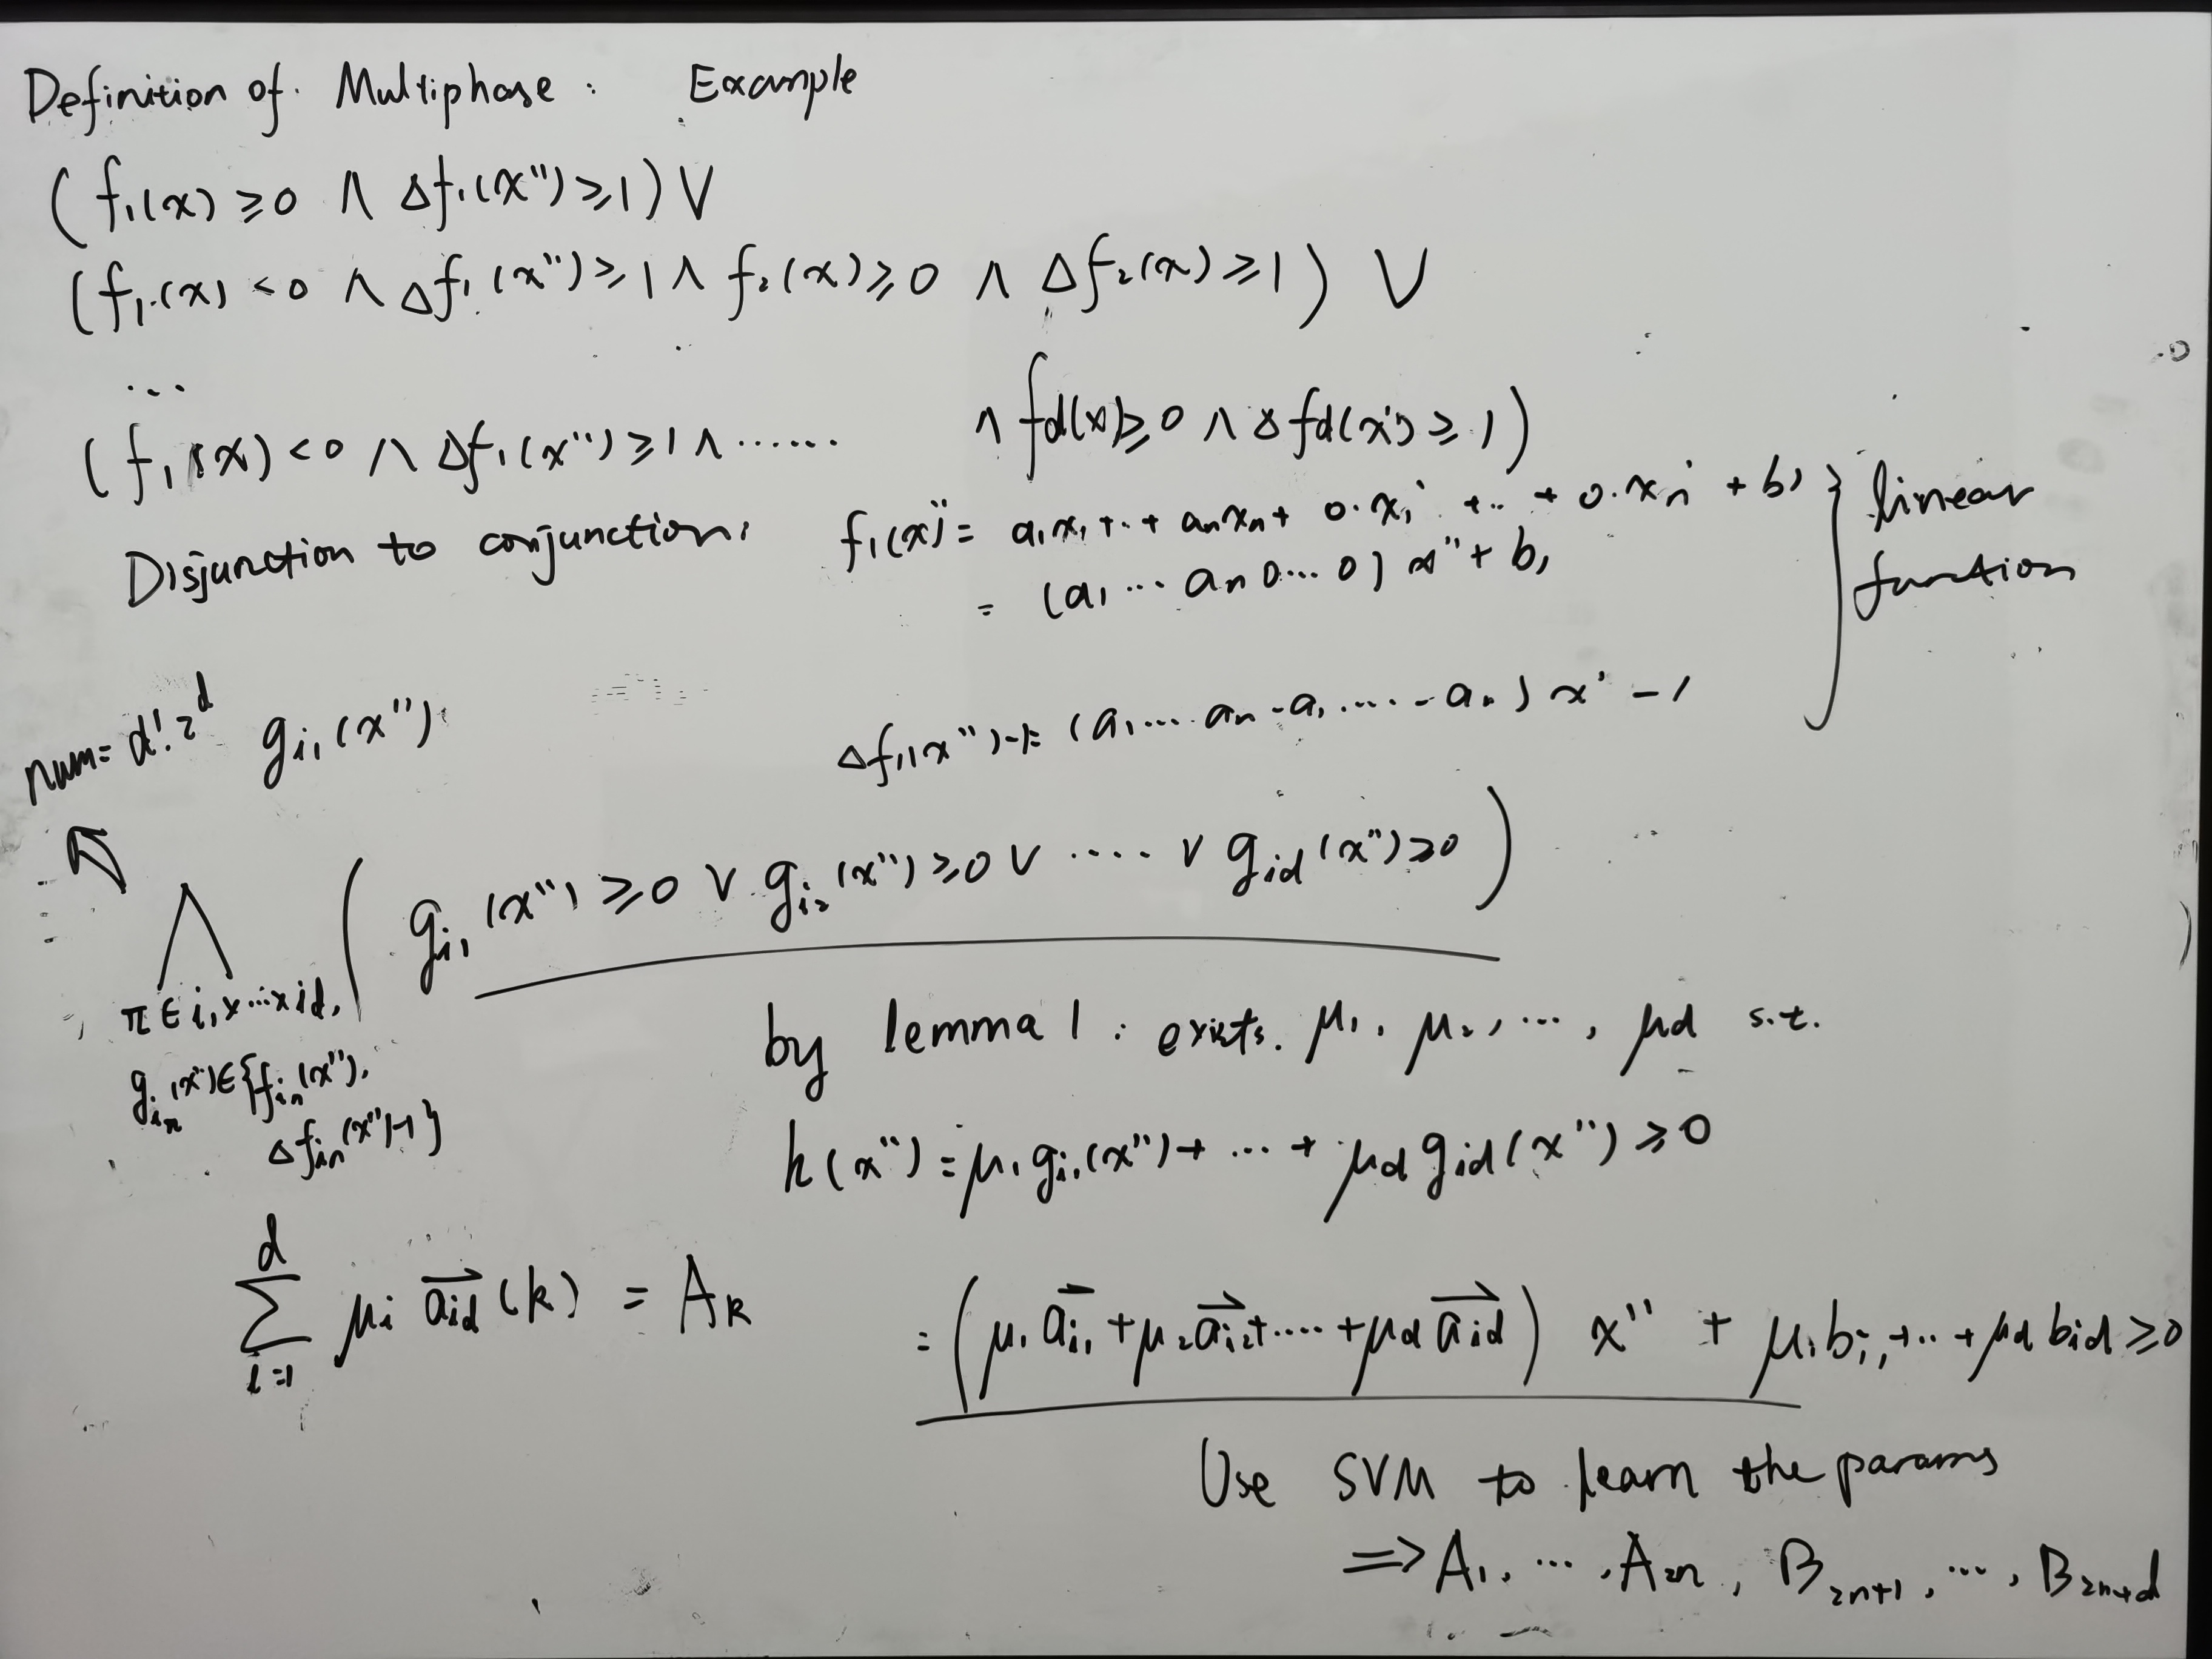
\includegraphics[scale = 0.08]{1.jpg}
%\end{center}

%\end{frame}
\begin{frame}\frametitle{Idea3: Use lemma 1 and SVM for synthesizing}
By definition of multiphase ranking function:
\[(f_1(x) \ge 0 \wedge \Delta f_1(x'') \ge 1 ) \vee \]
\[(f_1(x) < 0 \wedge \Delta f_1(x'') \ge 1 \wedge f_2(x) \ge 0 \wedge \Delta f_2(x'') \ge 1)\vee\]
\[\vee\cdots\vee\]
\[(f_1(x) < 0 \wedge \Delta f_1(x'') \ge 1 \wedge \cdots \wedge f_d(x) \ge 0 \wedge \Delta f_d(x'') \ge 1)\]

Two types of function: 
\begin{itemize}
\item $f_1(x'') = a_1x_1 + \cdots + a_nx_n + 0\cdot x_1' + \cdots + 0\cdot x_n' + b_1$

$ = (a_1, \cdots ,a_n, 0, \cdots, 0)x'' + b_1$
\item $\Delta f_1(x'') - 1 = (a_1, \cdots, a_n, 0, \cdots, 0) x'' + b_1'$
\end{itemize}

Let $f_{i_n} \in \{f_{i_n}, \Delta f_{i_n} - 1\}$ Rewrite the disjunction:
$\bigwedge_{\pi \in i_1 \times \cdots \times i_d} (g_{i_1}(x'') \ge 0 \vee g_{i_2}(x'') \ge 0 \vee \cdots \vee g_{i_d}(x'') \ge 0 )$
\end{frame}

\begin{frame}\frametitle{Idea3 Continue}
\[g_{i_1}(x'') \ge 0 \vee g_{i_2}(x'') \ge 0 \vee \cdots \vee g_{i_d}(x'') \ge 0 \]

Since $g_i$ is linear, by lemma 1 we got there exists $\mu_1, \cdots, \mu_n$ s.t.

\[\mu_1 g_{i_1}(x'') + \cdots + \mu_d g_{i_d}(x'') \ge 0\]
\[(\mu_1\vec{a_{i_1}} + \cdots + \mu_d \vec{a_{i_d}}) x'' + \mu_1 b_1 + \cdots + \mu_d b_{i_d} \ge 0\]
Then we can use SVM to learn the parameters.

\end{frame}

\begin{frame}\frametitle{Irrelevant Idea4}
Question: Is a partial ranking function useful? Here partial means only a part of the transitions of the loop are ranked but not all. Can we use this information to shrink the space we consider for generating recurrent set?



\end{frame}


\end{document}